\section{Extending the baseline model with preventive measures}\label{sec:extended_model}

In this chapter, I present the extensions made to the baseline model set out in Chapter~\ref{sec:baseline_model} to determine the impacts of preventive measures on a simulated population. The aims of this chapter correspond to Objectives~\ref{ro1} and \ref{ro2}: First, to create an extended model aligned to a realistic setting, and second, to assess the impacts of preventive measure use on disease spread. To accomplish this, I first empirically ground the baseline model using real-world data, and subsequently validate the extended model by conducting experiments and comparing the dynamics of the extended model to real-world observations.%to examine the impacts of preventive measure use on disease spread.

In the following sections, I first motivate why extensions to the baseline model are necessary to ground the model in a real-world scenario. Then, I describe the survey data used to inform the additional mechanisms in the extended model, and I outline the parameterisation process. Finally, I simulate hypothetical scenarios in the model and conduct data analysis to assess how various levels of preventive measure adoption can influence disease spread.

\subsection{Empirically grounded agent-based models}

Using quantitative and qualitative data to create empirically grounded agent-based models (ABMs) is a challenging task due to data constraints and the risk of over-specifying models \cite{janssen_empirically_2006}. When realism is desirable in ABMs, modellers typically use survey and time-series data to contextualise models to real-world systems \cite{polhill_using_2010, bruch_agent-based_2015, ghorbani_structuring_2015, canales_agent-based_2024}. However, aligning models to data requires incorporating sufficient realism to capture realistic patterns without over-complicating the model or obfuscating its tractability and analytic results \cite{bruch_agent-based_2015}. ABMs that retain their generality and simplicity with a data-driven design ideally achieve what \citet{bruch_agent-based_2015} call \q{low-dimensional realism,} in which models yield the usual benefits of the agent-based approach in addition to \q{empirical realism along one or two dimensions.}

Achieving low-dimensional realism is one goal of the extended model presented in this chapter due to the desire to investigate dynamics of preventive behaviours. Since psychological behaviour change theories are grounded in reality, a model that incorporates these theories should feature characteristics representative of a real-world setting. While the baseline agent-based model (ABM) from \citet{manore_network-patch_2015} incorporates realistic components of vector-borne disease (VBD) spread, the model architecture is intentionally general. Realistic features of the baseline model include heterogeneous environmental and geographic features, host mobility, and explicit vector dynamics. However, as \citet{manore_network-patch_2015} admit, the baseline model serves to showcase the \q{simple methodology} of the network-patch architecture, rather than function as a representative model of a specific VBD.

Another important process for aligning ABMs to empirical data is parameterisation. Using observational data to parameterise models with realistic parameter configurations is crucial for ABMs that simulate complex dynamics, especially disease transmission \cite{judson_modeling_2024}. However, parameterisation can be difficult for models at the individual level due to the large amount of data required, and the broad assumptions about populations that must be made \cite{canales_agent-based_2024}. For ABMs that incorporate preventive behaviours, modellers have previously used demographic information and behavioural survey data to derive parameter values that correspond to real-world values \cite{weston_infection_2018}.% Below, I take a similar approach by using data ... creating a scenario that is representative of a real-world setting.

Several methodologies have been proposed to formally integrate qualitative and empirical data into the design of ABMs. In their use of qualitative interview data for an ABM of land use change, \citet{polhill_using_2010} detailed how, at the time of writing, there was \q{no established methodology for implementing qualitative [data] in agent-based models.} In the study, this resulted in an ad hoc process of integrating qualitative insights into the ABM by reviewing findings and identifying corresponding code implementations. Since then, multiple methodologies have been formulated to interpret and structure data for integration within ABMs \cite{nespeca_methodology_2023}.

To align the baseline ABM to a real-world setting, I use the \q{Modelling Agent systems based on Institutional Analysis} framework (MAIA) \cite{ghorbani_maia_2013, ghorbani_structuring_2015}. Established as a framework for using qualitative data to integrate real-world phenomena into ABMs, MAIA has specifically gained traction for its ability to capture complex social phenomena through a set of five concepts. While MAIA has been criticised for lacking flexibility and only applying to certain ABM architectures in some cases \cite{nespeca_methodology_2023}, the framework still offers utility in its comprehensive nature, relevance to various domains, and built-in validation of implemented mechanisms from qualitative data.

The five concepts set out in the MAIA framework by \citet{ghorbani_maia_2013} are:

\begin{enumerate}[label=\textbf{\arabic*}.]
    \item \textbf{Collective structure.} What do agents represent and what are their collective attributes?
    \item \textbf{Constitutional structure.} What is the social context of agents---how do agents interact?
    \item \textbf{Physical structure.} What are the physical aspects of the real-world system recreated in the model?
    \item \textbf{Operational structure.} How is scheduling implemented for agents, what are the dynamics and relationships of the real-world system?
    \item \textbf{Evaluative structure.} Which concepts can be used to validate and measure the outcomes of the model?
\end{enumerate}

In the following section, I use MAIA to systematically describe the extensions to the baseline model.

\subsection{Methods}

In this section, I describe how qualitative and quantitative data were used to inform the extensions to the baseline model from Chapter~\ref{sec:baseline_model}. First, I describe the data sets chosen and explain why they are suitable for the purpose of extending the baseline model. Then, I detail the extensions made to the model and the parameterisation process. Finally, I outline the experiments run to validate the behaviour of the extended model against qualitative patterns observed in the study data.

\subsubsection{Description of data used}

To adapt the baseline model to a real-world scenario, I used empirical and qualitative data from three surveys of malaria activity within the Mondulkiri province, Cambodia \cite{pepey_mobility_2022, sandfort_forest_2020, vantaux_anopheles_2021}. There is a wealth of qualitative and quantitative VBD survey data available that could be used to inform ABMs for VBD spread. However, the data from the rural Mondulkiri province are appropriate for the following reasons: First, the data are diverse and complementary---the three surveys used here collected: (1) mobility patterns for inhabitants \cite{pepey_mobility_2022}; (2) behavioural and population characteristics of those inhabitants \cite{sandfort_forest_2020}; and (3) abundance statistics of mosquitoes in the area throughout different seasons \cite{vantaux_anopheles_2021}. Overall, these three dimensions---mobility, population characteristics, and vector abundance---can be used to independently inform different components of the baseline model.

A second benefit is that the data describe a single community with a scale appropriate for the baseline model. Approximately 17 villages in the \q{relatively small spatial scale} of the region were surveyed in \citet{sandfort_forest_2020}, which is aligned with the intended scale of the baseline model from \citet{manore_network-patch_2015} in which patches are stated to be \q{on the order of a building or a group of buildings.} Furthermore, with 4,200 surveyed participants, sample coverage was relatively high at just above 40\% of the total province population. Conveniently, the province is comprised of areas with heterogeneous spatial and environmental characteristics, and as a result, differing risk profiles for malaria infection. \citet{sandfort_forest_2020, vantaux_anopheles_2021} classified households as either being outside, on the fringe of, or inside the large forest surrounding the region, and concluded that the regions had distinct infection risk profiles.

All three studies collected various forms of data for these three distinct geographical regions (hereafter referred to as \textit{outside forest}, \textit{fringe forest}, and \textit{inside forest}). The population mobility study by \citet{pepey_mobility_2022} recorded daily movement patterns of forest-goers, a high-risk sub-population of the province. The entomological survey, on the other hand, investigated the temporal abundance and infectivity of \textit{Anopheles} mosquitoes over 60 days during the province's dry and rainy seasons \cite{vantaux_anopheles_2021}. The researchers used human- and cow-odour-baited traps placed across the land types to record mosquito frequency, biting rates, and the prevalence of malaria. Finally, the cross-sectional survey conducted by \citet{sandfort_forest_2020} tested inhabitants for malaria parasites via fingertip pricking and polymerase chain reaction (PCR) testing. The authors studied 2,351 households across 17 villages and classified their land type regions based on the amount of forest cover surrounding the village within a 750 m radius, as shown in Figure~\ref{fig:extended-model-i}. Behavioural characteristics (e.g., participants' habitual use of vector control tools, tendencies to travel to the forest) and population characteristics (e.g., age, household conditions) were recorded across these regions as part of the study.

Overall, these data present a unique opportunity to empirically and comprehensively ground the baseline model to inform agent mobility, population attributes, and vector dynamics within the model. To clarify, the goal of this extended model is not to accurately model malaria spread within the Cambodian region specifically, but rather to represent a real-world setting where a VBD outbreak could spread across a community with diverse behavioural attitudes and heterogeneous geographical properties. In the following sections, I describe the systematic process to adapt the results from the three studies to pursue the low-dimensional realism described by \citet{bruch_agent-based_2015}.

\begin{figure}[hbt!]
     \centering
     % \includegraphics[width=\textwidth]{figures/ch4/region_mapping_raw_fig.pdf}
     \resizebox{0.75\textwidth}{!}{
        \input{figures/ch4/region_mapping_raw_fig.pdf_tex}
     }
         \bcaption{Household locations and region groupings of the Mondulkiri province survey.}{Dots are households: Blue represents the outside forest region, green corresponds to the inside forest region, and pink is the fringe forest region. Indicative regions are drawn to demonstrate spatial heterogeneity. Adapted from \citet{sandfort_forest_2020}.}
    \label{fig:extended-model-i}
\end{figure}


\subsubsection{Description of model extensions}\label{sec:ch4-extensions}

As previously described, I use the MAIA framework to present the extensions that empirically ground the baseline model. Below, I emulate the approach used by \citet{ghorbani_structuring_2015} to list the concepts from MAIA, the insights from the data described above, and the corresponding model implementations.

\odd{Agents and their collective and constitutional attributes.}

In the extended model, agents belong to one of three roles: forest workers, field workers, or non-workers. In \citet{sandfort_forest_2020}, participants' occupations were found to influence their movement patterns and behaviour, such as their tendency to visit high-risk areas of infection (fields, plantations, and forests). Therefore, incorporating these risk groups into the model served to capture heterogeneous exposure rates within the population. The majority (75.86\%) of participants had work duties, with 24.14\% claiming no work in the past two months. While most workers listed their occupation as either a forest or field worker, the remaining workers cited having \q{other} jobs. To incorporate working roles in the model yet retain simplicity, these responses were omitted, and forest and field worker amounts were proportionally scaled as shown in Table~\ref{tab:data-occupations}. The resulting split of working groups was 5\% forest workers, 71\% field workers, and 24\% non-workers.

\begin{table}[h]
    \centering
    \begin{adjustbox}{center}
        \begin{tabular}{lcccc} \toprule
            Work type & Number of workers & Proportion & Scaled number of workers & Proportion \\ \midrule
            Deep forest & 145 & 3\% & 207 & 5\% \\
            Cassava field & 2,085 & 50\% & 2,979 & 71\% \\
            Other & 956 & 23\% & 0 & 0\% \\
            No work & 1014 & 24\% & 1,014 & 24\% \\ \midrule
            Total & 4,200 & 100\%& 4,200 & 100\% \\ \bottomrule
        \end{tabular}
    \end{adjustbox}
    \bcaption{Derivation of risk group proportions.}{\q{Other} workers were omitted from the data set and proportions were redistributed among field and forest workers. Percentages and scaled figures are rounded to the nearest whole numbers.}
    \label{tab:data-occupations}
\end{table}

Heterogeneous risk exposure owing to occupation was also indirectly recreated in the model. Upon initialisation, each agent is randomly assigned a working role according to the final proportions in Table~\ref{tab:data-occupations}. All agents are assigned a \q{home node} as the initial node they begin the simulation in, and working agents (forest or field workers) have an additional \q{work node} they commute to. More information on the mobility and scheduling of agent risk groups is provided further below. Ultimately, an agent's working role influences their movement patterns and activities in the model, thereby exposing workers to different levels of infection risk.

\odd{Agents and the physical structure of the extended model.}

% The extended model has three patches: outside forest, fringe forest, and inside forest. These patches directly correspond to the three land types defined in \citet{sandfort_forest_2020}, as the surveyed regions were spatially and environmentally distinct. As concluded by all three studies, malaria exposure risk was correlated with activities and travel near forested areas \cite{pepey_mobility_2022, vantaux_anopheles_2021, sandfort_forest_2020}. The outside forest patch had the lowest infection risk, the fringe forest had a higher infection risk, and the inner-forest region had the highest infection risk. Evidently, the distinct variation in patch exposure risk is an important factor of the province's environment, and thus an important environmental characteristic to encode in the extended model. Aerial photography of the survey area is shown in Figure~\ref{fig:extended-model-i} with households and groupings of the land types.

The extended model has three patches: the outside forest, fringe forest, and inside forest. These patches correspond directly to the three distinct land types defined in \citet{sandfort_forest_2020} shown in Figure~\ref{fig:extended-model-i}. Malaria exposure risk was distinct between the three regions in the survey data, and infection risk was correlated with proximity to forested areas: The region outside the forest had the lowest infection risk, the fringe forest region had a higher infection risk, and the inside forest region had the highest infection risk \cite{pepey_mobility_2022, vantaux_anopheles_2021, sandfort_forest_2020}. Incorporating this geographical and environmental heterogeneity of patches in the extended model was important as different infection risk profiles of patches can directly or indirectly influence disease spread.

% -> TS: There are three patches in the extended model.
% -> SS:
%     - These patches correspond to the land types defined in Sandfort, shown in Figure 1.
%     - According to the study, these regions have distinct infection risk profiles.
%     - Outside < fringe < inside.
% -> CS: This is important to model as this incorporates heterogeneous environmental characteristics that may directly and indirectly affect disease spread.

The patches in the extended model contain different location types informed by the survey data. All patches contain household nodes that agents \q{sleep} in by remaining stationary within these nodes during nighttime hours (further explained in the next section). As in the baseline model, these household nodes are distributed among the three patches according to patch densities (a derivation is provided later in Section~\ref{ch4:parameterisation}). As shown in the layout of the extended model in Figure~\ref{fig:extended-model-ii}, the outside and fringe forest patches both contain one extra node representing a cassava field site (or plantation) which field workers commute to. Similarly, the inside forest patch contains an additional node representing a forest work site travelled to by forest workers. Importantly, not all forest workers live in the forest, as work-related activities in the forest were found to be a source of income for inhabitants across the province \cite{sandfort_forest_2020, pepey_mobility_2022}. There is no field site in the inside forest patch as the geographic properties of the area indicate little to no field cover \cite{sandfort_forest_2020}. While fields and plantations are distinct land uses, \citet{sandfort_forest_2020} and \citet{vantaux_anopheles_2021} highlight few differences between their mobility patterns and infection risk, so the land categories were aggregated in the extended model.

\begin{figure}[hbt!]
     \centering
     \resizebox{0.95\textwidth}{!}{
        \input{figures/ch4/exml.tex}
     }
     \bcaption{Extended model layout and mobility.}{The light blue patch ($k=0$) is the outside forest patch where 85\% of agents live. The pink patch ($k=1$) is the fringe forest patch, and the green patch ($k=2$) is the inside forest patch. Solid lines between households represent edges in the underlying network. \textbf{(i)} Field workers in the outside forest patch commute to the field site node for work. \textbf{(ii)} Field workers in the fringe and inside forest patch commute to the field site node in the fringe forest patch. \textbf{(iii)} Forest workers from all patches commute to the forest site node for work. \textbf{(iv)} Non-workers move randomly throughout connected household nodes in their own patch. Icons are provided by the Noun Project \cite{rizal_forest_nodate, tegalsari_household_nodate, harianto_crops_nodate}.}
     \label{fig:extended-model-ii}
\end{figure}

%As 2,351 households were surveyed, the same number of household nodes are added to the model, distributed over the three patches. The derivation of these densities is given in Section~\ref{ch4:parameterisation}.

%This layout of the extended model is demonstrated in Figure~\ref{fig:extended-model-ii}.

\odd{Agents and the operational structure of the extended model.}

The scheduling of agent movement in the extended model is aligned with the routines of participants described in \citet{sandfort_forest_2020} and \citet{vantaux_anopheles_2021}. As shown in Figure~\ref{fig:extended-model-scheduling}, agent movement patterns are based on their occupation and location: At 8am, working agents commute to their corresponding work node. Forest workers commute to the forest site node while field workers commute to their nearest field site node (field workers in the inside forest patch travel to the fringe forest patch). Non-workers employ the random movement model defined in \citet{manore_network-patch_2015} during the daytime to move randomly throughout households that are within their home patch and connected via the underlying network. At 8pm, all agents return to their home node where they remain until 8am the next day, when the process is repeated. Agent movement patterns are repeated daily as agent routines are intended to be a simplified recreation of the mobility dynamics described in \citet{pepey_mobility_2022}.

\begin{figure}[hbt!]
     \centering
     \adjustbox{width=1.1\textwidth,center}{
        \input{figures/ch4/agent-mosquito-scheduling.tex}
     }
     % \includegraphics[width=\textwidth]{figures/ch4/scheduling.png}
     \bcaption{Scheduling of agents and mosquitoes over one day.}{Mosquitoes have a heightened maximum number of bites per time step ($\sigma_v$) by a factor of four from 6pm--10am. Agents are awake from 8am--8pm, creating four hours (two time steps) of overlap with heightened mosquito activity time. Immediately prior to sleeping, agents decide whether to use an ITN or not.}
    \label{fig:extended-model-scheduling}
\end{figure}

In addition to agent mobility, vector activity in the extended model varies depending on the time of day. In the abundance study by \citet{sandfort_forest_2020}, 20\% of mosquito biting activity occurred between 6am--6pm across all regions in the province, meaning mosquito activity was heightened by a factor of approximately 4 outside of these hours. Similarly, \citet{pepey_mobility_2022} noted an increased prevalence of mosquitoes during dusk, nighttime, and dawn. To incorporate this varying mosquito activity in the extended model, mosquitoes have a heightened presence from 6pm--10am to overlap with agents' daily schedules by four hours. This is aligned with biting rate figures from the abundance study shown in Figure~\ref{ch4:biting-rate-abundance}, where mosquito prevalence only significantly fell between 10am--6pm. In the extended model, heightened mosquito activity was simulated by temporarily increasing the maximum number of bites per vector each time step ($\sigma_v$) by 4x between 6pm--10am.

% $\sigma_v$ is representative of mosquito biting activity and is used in the biting rate derivation \eqref{eq:bites}, meaning it indirectly impacts the force of infection \eqref{eq:lambda-v} on agents.

\begin{figure}[hbt!]
     \centering
     \includegraphics[width=1.1\textwidth]{figures/ch4/vantuax_fig2.png}
         \bcaption{Average number of Anopheles mosquitoes collected in traps per hour over one day.}{Two odour-baited traps (cow-odour-baited double net traps (CBNTs) and human-odour-baited double net traps (HBNTs)) were set across the collection sites plotted in Figure~\ref{fig:collection-sites}. Taken from \citet{vantaux_anopheles_2021}.}
    \label{ch4:biting-rate-abundance}
\end{figure}

The final extension made to the baseline model was the inclusion of insecticide treated bed nets (ITNs) as preventive measures. ITNs used during sleep---the hours of highest mosquito activity---protect against infection through physical (net material) and chemical (insecticide) means. Out of 4,200 participants, 3,880 (92.4\%) claimed they had slept under a bed net the previous night of the survey, although only 41\% of bed nets were treated with insecticide \cite{sandfort_forest_2020}. Virtually all (99.3\%) households in the survey had access to bed nets with an average of just under three bed nets per household, and 90\% of participants said they slept under a net every night \cite{sandfort_forest_2020}. In contrast to other preventive measures in the region, such as mosquito repellent or indoor residual spraying, ITNs are readily available, easy to use, and supported by a large body of literature on their use as a preventive measure. Overall, these factors made ITNs an appealing preventive measure to include in the extended model.

Each night in the simulation, agents decide whether to sleep under an ITN. At 8pm, every agent generates a uniform random number $\theta\in[0,1]$ and employs an ITN if $\theta<p_{\text{ITN}}$. When used, ITNs dampen the probability of infection from mosquitoes by 99\% during agent sleeping hours (8pm--8am). In other words, the transition probability $\mathbb{P}(S_h\to E_h)$ in equation \eqref{eq:agents} is reduced to $0.01\times\mathbb{P}(S_h\to E_h)$. While this effect is likely overstated, the high efficacy of ITNs in the model creates an ideal scenario as a reference point for disease mitigation when ITNs are almost entirely effective. A constant efficacy value of ITNs also helps isolate the impacts of later extensions to the model made in Chapter~\ref{sec:bcts} regarding behaviour change theories.

\subsubsection{Parameterisation of model}\label{ch4:parameterisation}

I used data from the three surveys of the Mondulkiri province to parameterise the extended model. Below, I detail the methodology for deriving parameter values from the data sets:

\begin{description}
    \item[Two-hour time steps.] Time steps in the extended model ($\Delta t$) are two hours. Compared to the six-hour time steps in \citet{manore_network-patch_2015}, the higher granularity creates two daily time steps (8am--10am and 6pm--8pm) during which mosquito activity is heightened but agents are awake (and thus cannot use ITNs). Including this temporal dynamic was important as \citet{pepey_mobility_2022} observed that mosquitoes were often active in the region \q{outside the hours of bed net use} during the early morning and night.
    \item[Patch, household, and agent numbers.] As mentioned above, the outside, fringe, and inside forest patches correspond to the heterogeneous geographical and environmental properties of the region. In the extended model network, 2,351 household nodes are defined and populated with 10,053 agents to align with the population statistics from \citet{sandfort_forest_2020}. Using supplementary data from the study, I calculated the density of households per region and determined that 85\% of households were located in the outside forest region, 8\% in the fringe forest region, and 7\% in the inside forest region. Upon model initialisation, these densities are used to distribute agents among households (as described in Section~\ref{oddsec:initialisation}).
    \item[Patch mosquito carrying capacities.] To derive the number of mosquitoes per patch, I used supplementary data from \citet{vantaux_anopheles_2021} to first compute mosquito densities across the three regions and chose carrying capacities $K_v^{(k)}$ for each patch $k\in\{0,1,2\}$ to align with the infection dynamics in \citet{manore_network-patch_2015}. Figure~\ref{fig:collection-sites} plots the collection sites from \citet{vantaux_anopheles_2021} in the context of the survey region from \citet{sandfort_forest_2020}. I mapped these collection sites to the coloured land classifications by \citet{sandfort_forest_2020} (outside, fringe, and inside forest) based on their proximity to neighbouring classified households.

    \begin{figure}[hbt!]
         \centering
         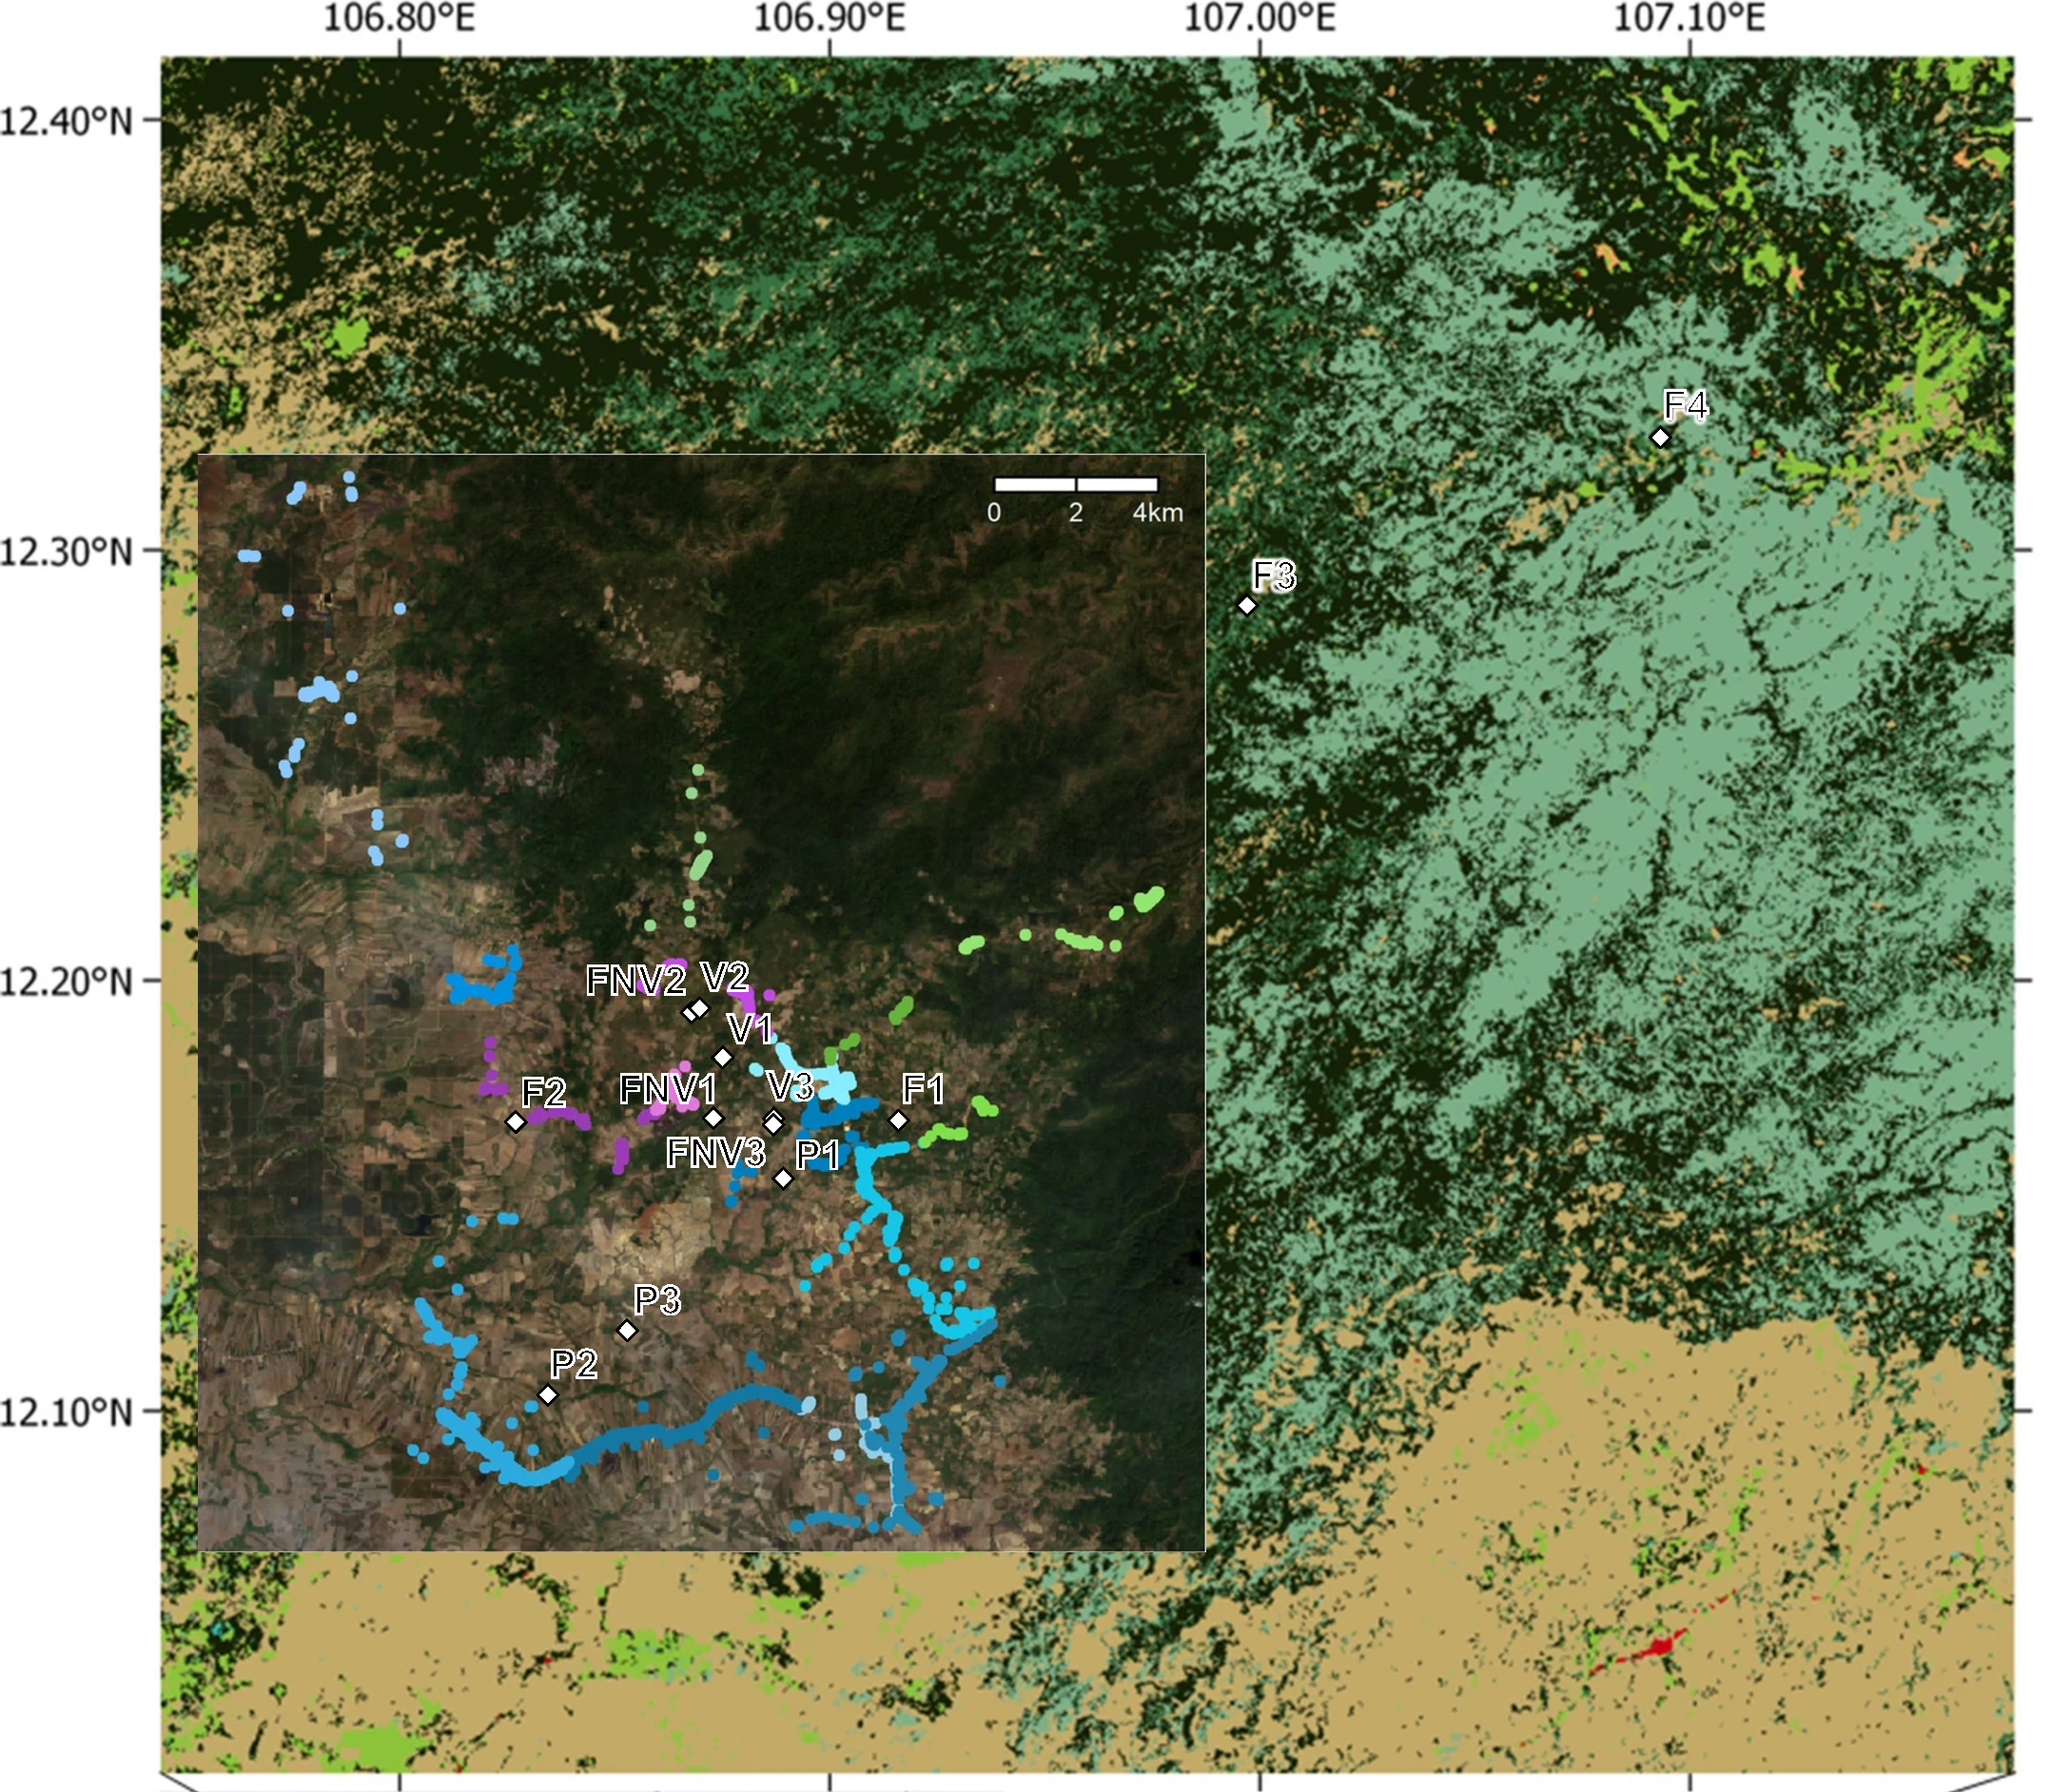
\includegraphics[width=\textwidth]{figures/ch4/collection-regions.pdf}
             \bcaption{Collection sites of mosquitoes overlayed on survey region.}{Coloured dots represent survey locations from \citet{vantaux_anopheles_2021}, whereas diamonds represent collection sites. Sites include forest locations (F1--4), forest-near-village locations (FNV1--3), villages (V1--3), and plantations (P1--3). Larger map taken from \citet{vantaux_anopheles_2021} and smaller overlaid map from \citet{sandfort_forest_2020}.}
        \label{fig:collection-sites}
    \end{figure}

    Village and plantation collection sites (V1–3, P1–3) lied in the outside forest region, whereas the forest-near-village collection sites (FNV1--3) were representative of the fringe forest region. The second forest collection site (F2) was re-classified to the fringe forest region due to its proximity to fringe forest households, and the other forest classification sites (F1, F3, F4) represented the inside forest region. Table~\ref{tab:mosquito-collection} shows the aggregation process to derive the density of mosquitoes per region.

    \begin{table}[hbt!]
        \centering
        \begin{adjustbox}{center}
            \begin{tabular}{ccccc} \toprule
                \multirow{2}{*}{Region} & \multirow{2}{*}{Site} & \multirow{2}{*}{\shortstack[c]{Mosquitoes\\collected}} & \multirow{2}{*}{\shortstack[c]{Average mosquitoes\\per site}} & \multirow{2}{*}{Density ratio} \\
                & & & & \\ \midrule
                \multirow{4}{*}{Inside forest} & F1 & 185 & \multirow{4}{*}{86.33} & \multirow{4}{*}{3.24} \\ 
                 & F3 & 53 & ~ & ~ \\ 
                 & F4 & 21 & ~ & ~ \\ 
                 & \textbf{Total} & 259 &  &  \\ \midrule
                \multirow{3}{*}{Fringe forest} & F2 & 231 & \multirow{3}{*}{78.50} & \multirow{3}{*}{2.94} \\
                 & FNV1–3 & 83 & ~ & ~ \\ 
                 & \textbf{Total} & 314 &  &  \\ \midrule
                \multirow{3}{*}{Outside forest} & V1–3 & 43 & \multirow{3}{*}{26.67} & \multirow{3}{*}{1} \\ 
                 & P1–3 & 117 & ~ & ~ \\ 
                 & \textbf{Total} & 160 &   &   \\ \bottomrule
            \end{tabular}
        \end{adjustbox}
        \bcaption{Mosquito collection site statistics and density derivation.}{Collection sites were mapped to regions and mosquito figures were aggregated. Then, densities were derived based on the average number of mosquitoes collected within the region. Data were sourced from supplementary data in \citet{vantaux_anopheles_2021}.}
        \label{tab:mosquito-collection}
    \end{table}

    The resulting ratio of mosquito densities across patches was $1 : 2.94 : 3.24$, which was rounded to $1 : 3 : 3.5$ to eliminate implausible precision. The corresponding patch carrying capacities were thus $K_v^{(1)}=3K_v^{(0)}$ and $K_v^{(2)}=3.5K_v^{(0)}$, where $k=0$ is the outside forest patch, $k=1$ is the fringe forest patch, and $k=2$ is the inside forest patch. I chose $K_v^{(0)}$ such that the extended model had the same approximate timing of peak epidemic activity as the high movement baseline scenario from \citet{manore_network-patch_2015} (approximately 100 days, as shown in Figure~\ref{fig:validation-2}). This alignment, shown in Figure~\ref{fig:k_v_candidates}, effectively calibrated the extended model to reproduce the infection dynamics of the baseline model. The resulting patch carrying capacities were $K_v^{(0)} = 2700, K_v^{(1)}= 8100, K_v^{(2)}=9450$.

    \begin{figure}[hbt!]
         \centering
         \includegraphics[width=\textwidth]{figures/ch4/k_v_candidates.pdf}
         \vspace{-1cm}
         \bcaption{Distribution of epidemic peak timings for different $K_v^{(0)}$ values.}{$K_v^{(0)}=2700$ was found to most closely align with the high movement scenario from \citet{manore_network-patch_2015} of approximately 100 days. Results from $K_v^{(0)}$ values 10\% below and above this value are shown on the left and right respectively. Median values for groups from left to right were: 102, 100, and 97 days.}
        \label{fig:k_v_candidates}
    \end{figure}
    
    \item[Heterogeneous location exposure parameters.] In the survey data, agents' exposure to mosquitoes in fields and forests was different compared to households. To capture this in the extended model, I adjusted the location exposure parameter $\alpha_j$. According to supplementary data from \citet{sandfort_forest_2020}, 57\% of participants live in households with windows, so I set $\alpha_{\text{household}}=0.43$ to capture this partial protection in most households. Field and forest work sites are entirely exposed to the outdoors, so I assumed $\alpha_{\text{field}}=\alpha_{\text{forest}}=1.0$ in the extended model.
\end{description}

\subsubsection{Indicators of model validity}\label{maiasec:questions}

To assess the validity of the extended model, I compared the observed trends in the Cambodia data to the behaviour of the extended model under similar conditions. This section in the MAIA framework proposes integrating validation into the qualitative data alignment process by identifying indicators of the extended model's usability and validity \cite{ghorbani_maia_2013}. To holistically validate the extended model's behaviour, I propose the following dynamics to be investigated later in this chapter during experimentation:

\begin{description}
    \item[Mosquito biting rates and exposure times.] Since mosquito activity is highest during the hours of dusk, nighttime, and dawn, most agents should be infected during these hours.
    \item[Heterogeneous infection risk across patches.] In \citet{vantaux_anopheles_2021}, the forest regions had six times more infectious mosquito bites compared to villages. Therefore, in the extended model, infections in the fringe and inside forest patches should be substantially higher than those in the outside forest patch.
    \item[ITNs decrease infections during the night.] Increasing $p_{\text{ITN}}$ should lead to higher ITN adoption across the province, and thus a decrease in overall transmission.
    \item[Heterogeneous occupation exposure rates.] \citet{sandfort_forest_2020} found that prevalence of malaria was highest in forest workers (25.5\%), lower in field workers (7.2\%), and lowest in non-workers (1.5\%). The risk profiles of occupations in the extended model should reflect this ordering.
\end{description}

\subsubsection{Experiments and sensitivity analysis}

I conducted various experiments and sensitivity analysis to address the validation criteria proposed in Section~\ref{maiasec:questions}. First, I ran the model 50 times with no agent ITN use ($p_{\text{ITN}}=0$) to investigate the dynamics of the parameterised extended model without interventions. Then, I visualised the behaviour of the model to investigate the validity considerations around mosquito biting rates, infection timings, infection risk, and varying risk profiles of occupational groups. Next, I varied ITN use to assess the impacts of different preventive measure compliance rates in the population. Specifically, I varied the probability an agent slept under an ITN ($p_{\text{ITN}}$) across three values: 0\%, 50\%, and 100\%. Finally, I conducted sensitivity analysis to quantify the effects of heterogeneous mosquito densities across patches by simulating three distinct scenarios:

\begin{description}
    \item[1. Derived patch carrying capacities.] I ran the model with the values for $K_v^{(0)}$, $K_v^{(1)}$, and $K_v^{(2)}$ derived using empirical data from \citet{vantaux_anopheles_2021} above.
    \item[2. Equal total volume, distributed uniformly.] Preserving the total number of mosquitoes from the derived $K_v^{(k)}$ values (i.e., $\sum_{k}{K_v^{(k)}}$), I distributed all mosquitoes over the three patches uniformly, i.e., $\forall k : K_v^{(k)}=\frac{1}{3}\sum_{k}{K_v^{(k)}}$.
    \item[3. Equal total volume, distributed with equal vector-to-host ratios.] Similar to the second scenario, using $\sum_{k}{K_v^{(k)}}$, I instead distributed mosquitoes according to the patch densities such that all patches had an equal vector-to-host ratio (i.e., $K_v^{(0)}/N^{(0)}_h=K_v^{(1)}/N^{(1)}_h=K_v^{(2)}/N^{(2)}_h$ (where $N^{(k)}_h$ denotes the number of agents belonging to the $k^{\text{th}}$ patch).
\end{description}

All other parameters used during experiments which were not derived in the previous sections remained the same as in the baseline model (see Appendix~\ref{appendix:manore-abm} for reference).

\subsection{Results}\label{sec:extended-model-results}

In this section, I present the results from the experiments described above. First, I describe the default behaviour of the model over 50 simulations without any variation in parameters. The purpose of this is to validate whether the expected dynamics described in Section~\ref{maiasec:questions} were observed when running the extended model. Next, I discuss the impacts of varying ITN adoption ($p_{\textsc{ITN}}$) of agents within the extended model. Finally, I investigate how heterogeneous mosquito densities across patches ($K_v$) affected disease spread.

\subsubsection{Validation of extended model}\label{sec:extended-model-validation}

\begin{figure}[htb!]
     \centering
     \includegraphics[width=.9\textwidth]{figures/ch4/no_itn_disease_dynamics.pdf}
     \bcaption{Agent disease dynamics over time.}{Solid lines represent results from the most representative model run\protect\footnotemark. Shaded bands around lines represent minimum and maximum values across all model runs\protect\footnotemark.}
    \label{fig:ch4res-overall}
\end{figure}

\newcounter{savefootnote}% Ensure the savefootnote counter exists

\setcounter{savefootnote}{\value{footnote}}% Store footnote counter
\addtocounter{footnote}{-1}% Decrease the footnote counter by 1
\footnotetext{I determine the most representative model run by choosing the result that minimises the sum of Euclidean distances across all other model runs.}

\setcounter{footnote}{\value{savefootnote}}% Restore the footnote counter
\footnotetext{Shaded bands around solid lines represent minimum and maximum values across all model runs in all other figures throughout this thesis, unless explicitly stated otherwise.}

Across the 50 model runs without any variation in parameters, $92.8\% \pm 0.5\%$ of agents were infected with disease, on average. Figure~\ref{fig:ch4res-overall} demonstrates the agent SIR dynamics across all model runs. Mosquito dynamics were heterogeneous across patches due to variable vector-to-host ratios, as shown in Figure~\ref{fig:ch4res-mosquito-dynamics}. Infection in the outside forest patch peaked the latest compared to the fringe and inside forest patch due to the low density of mosquitoes relative to a large (85\% of total) host population. Unlike the outside forest patch, the fringe and inside forest patches had steepened infection curves, and as a consequence, higher forces of infection on mosquitoes ($\lambda_v$) during the day and night. Unsurprisingly, nighttime $\lambda_v$ values were consistently higher than their daytime values due to heightened mosquito activity which caused higher biting rates, and thus a higher chance of mosquito infection during the hours of dusk, nighttime, and dawn.

\begin{figure}[hbtp!]
     \centering
     \adjustbox{width=1.1\textwidth,center}{%
        \includegraphics{figures/ch4/no_itn_mosquito_dynamics.pdf}
     }
     \bcaption{Mosquito disease dynamics across patches over time.}{SEI dynamics for mosquitoes are shown in the top row. Forces of infection on vectors ($\lambda_v$) are shown on the bottom row. Nighttime (when mosquito activity is heightened by 4x) forces of infection were always higher than daytime values. Because the outside forest patch did not quickly reach infection saturation, dynamics are spread out over the 200-day time frame.}
    \label{fig:ch4res-mosquito-dynamics}
\end{figure}

\begin{figure}[htb!]
     \centering
     \includegraphics[width=.9\textwidth]{figures/ch4/no_itn_cum_infected_agents.pdf}
     \bcaption{Cumulative infected agents across patches.}{Compared to the slower progression of the outside forest patch, the fringe and inside forest patches reached saturating levels of infection by day 60--65 due to their high vector-to-host density ratios.}
    \label{fig:ch4res-cum-infections}
\end{figure}

\begin{figure}[htb!]
     \centering
     \adjustbox{width=1.1\textwidth,center}{%
        \includegraphics{figures/ch4/no_itn_freq_infection.pdf}
    }
     \bcaption{Frequency of infection times and biting rates.}{Infection times (blue bars) were aggregated across all model runs and are shown in 24-hour format. Biting rates (black lines) are shown for one model run as the variation in biting rates was minimal. Values are highest when agents are exposed (at work) and mosquito activity is heightened by 4x during 6pm--10am.}
    \label{fig:ch4res-infection-day}
\end{figure}

\begin{figure}[hbt!]
     \centering
     \includegraphics[width=0.85\textwidth]{figures/ch4/no_itn_agent_infection_cum_occupation.pdf}
     \bcaption{Proportion of infected agents over time by occupation.}{\textbf{(i)} Infection proportions per risk group. \textbf{(ii)} Cumulative infection proportions per risk group. Forest workers reached saturating infection levels quickly due to their constant high exposure to mosquitoes. Field workers were more exposed to mosquitoes than non-workers, and thus experienced slightly higher rates of infection.}
    \label{fig:ch4res-risk-profiles}
\end{figure}

One interesting result was that the highest-risk inside forest patch had lower nighttime $\lambda_v$ values compared to the fringe forest patch. This was due to the patch's slightly smaller host population, a lower proportion of fully exposed workers, and the fact that forest workers tend to live in the outside or fringe forest patches, meaning they leave the inside forest patch to return home after work, reducing the concentration of infected agents in the patch, thus lowering $\lambda_v$. As shown in Figure~\ref{fig:ch4res-cum-infections}, infections across the fringe and inside forest patches typically saturated the host populations quickly in comparison to the slower rate of agent infection within the outside forest patch.

In the simulation, infection risk was also heterogeneous according to the time of day. Figure~\ref{fig:ch4res-infection-day} conveys how the 4x heightened mosquito activity during dusk, nighttime and dawn led to increased biting rates across all patches, disproportionately affecting the fringe and inside forest patches due to their high mosquito density. As a result of higher biting rates, agent infection mostly occurred in the late afternoon to early morning, and was most prevalent when mosquitoes were more active but agents were still at work (8--10am and 6--8pm). This high prevalence of infection during the nighttime despite protection from indoor household environments highlights the importance of vector control tools that limit contact rates during this time (such as ITNs).

\begin{figure}[hbt!]
     \centering
     \includegraphics[width=0.8\textwidth]{figures/ch4/no_itn_exposure_location.pdf}
     \bcaption{Frequency of agent infection locations by occupation.}{Infection counts in locations are aggregated across all model runs. Almost all forest workers were exposed at forest sites, compared to field workers who were mostly exposed at home. Non-workers were only ever exposed at home.}
    \label{fig:ch4res-inf-locations}
\end{figure}

Disease transmission was significantly different across agent occupations. Forest workers were consistently fully infected before halfway through the simulation, whereas infections for field and non-workers typically plateaued by the end of the simulation. As evidenced by Figure~\ref{fig:ch4res-risk-profiles}, the higher mosquito exposure of field workers led to a higher average infection count compared to the non-working population. Despite their frequent exposure to mosquitoes, most field workers (55.3\%) were infected while sleeping at home instead of within a field work site (38.1\%), as shown in Figure~\ref{fig:ch4res-inf-locations}. Forest workers, on the other hand, were overwhelmingly infected in their place of work (89.0\%) compared to their households (10.5\%)\footnote{These proportions suggest that across all model runs, only 0.5\% of forest workers remained uninfected by the end of the simulation.}.

\subsubsection{Impacts of preventive measure adoption}\label{sec:extended-model-p-itn-impacts}

\begin{figure}[htb!]
     \centering
     \includegraphics[width=0.85\textwidth]{figures/ch4/itn_agent_infection_p_use.pdf}
     \bcaption{Proportion of agents infected over time for different levels of ITN use.}{\textbf{(i)} Proportion of agents infected over time. \textbf{(ii)} Cumulative proportion of agents infected over time. Although no level of ITN adoption led to disease eradication, increasing ITN adoption from 0\% to 50\% led to a 15--20\% decrease in total infections on average, while 100\% adoption rates significantly reduced total infection counts to $<$40\% in all runs.}
    \label{fig:ch4res-itn-dynamics}
\end{figure}

\begin{figure}[htb!]
     \centering
     \adjustbox{width=1.2\textwidth,center}{%
        \includegraphics{figures/ch4/itn_risk_groups.pdf}
    }
     \bcaption{ITN use impacts on infected agents by occupation.}{The top row conveys infections over time, whereas the bottom row shows cumulative infections within each occupation. Forest workers were the least affected by ITN use due to their exposure, while field and non-workers greatly benefitted from adopting ITNs, approximately halving disease cases in both occupational groups.}
    \label{fig:ch4res-inf-occupations}
\end{figure}

As expected, ITN use drastically decreased disease spread. As shown in Figure~\ref{fig:ch4res-itn-dynamics}, increasing ITN use delayed the first peak of disease spread and flattened the second wave of disease. In the complete compliance case ($p_{\text{ITN}}=1.0$), ITNs reduced infection counts across simulations to under 40\% (from $>90\%$) and prevented the momentum of the first wave of disease from leading to a severe second wave, as in the 0\% and 50\% ITN adoption scenarios. That being said, all three scenarios of ITN use had an initial peak in infections between days 50--100.

\begin{figure}[htb!]
     \centering
     \adjustbox{width=1.2\textwidth,center}{%
        \includegraphics{figures/ch4/itn_freq_infection.pdf}
    }
     \bcaption{Frequency of infection times across ITN adoption rates.}{Infection times were aggregated across all model runs and are shown in 24-hour format. As ITN adoption increased, infections were concentrated during daytime hours of exposure.}
    \label{fig:ch4res-itn-infection-day}
\end{figure}

\begin{figure}[htb!]
     \centering
     \adjustbox{width=1.3\textwidth,center}{%
        \includegraphics{figures/ch4/itn_exposure_locations.pdf}
    }
     \bcaption{Agent exposure locations by risk group and ITN adoption.}{Infection counts in locations were aggregated across all model runs. As ITN adoption increased, field workers and non-workers experienced less infections at home, but forest workers remained relatively unaffected.}
    \label{fig:ch4res-itn-locations}
\end{figure}

The breakdown of infections by occupations in Figure~\ref{fig:ch4res-inf-occupations} demonstrates that these early peaks were due in part to the rapid infection of forest workers. When ITN use was increased, the rate of infection among field and non-workers was substantially lower, however the working population in the forest was relatively unaffected. This is not surprising given that forest workers were rarely infected in their households as shown in Figure~\ref{fig:ch4res-inf-locations}, so the impact of using ITNs was understandably diminished compared to field and non-workers.
% due to the single forest site location in the high-risk inside forest patch. 

Increasing ITN use led to higher daytime infection rates and more concentrated disease spread within work site locations. Figure~\ref{fig:ch4res-itn-infection-day} shows how increasing ITN use decreased infection during nighttime hours but concentrated disease spread during the daytime. Notably, infections grew most in the early morning and late afternoon hours compared to the relatively stable (but increasing) infections within mid-late daytime hours. Corresponding with the decrease in nighttime infections, agents were less likely to be infected in households as ITN use increased. As shown in Figure~\ref{fig:ch4res-itn-locations}, non-worker infections dropped from 89.0\% with no ITN use to 25.5\% in the total compliance scenario. Field workers similarly saw infections drop from 55.4\% without ITN use to 34.1\% in the half compliance scenario, and virtually no infections occurred within households in the full compliance case. As noted earlier, however, forest workers benefitted the least from ITNs, as only 10.5\% of forest worker infections originally occurred in households.


\subsubsection{Impacts of heterogeneous mosquito densities}

\begin{figure}[htb!]
     \centering
     \adjustbox{width=0.9\textwidth,center}{%
        \includegraphics{figures/ch4/k_v_distribution_epidemic_peak.pdf}
    }
     \bcaption{Distribution of epidemic peak timings across patch carrying capacity scenarios.}{\q{Derived} indicates the empirically derived carrying capacity values, whereas the two \q{equal} experiments are more homogeneous across patches. As mosquito distribution was more equal across patches, so were epidemic dynamics.}
    \label{fig:ch4-k-v-timings}
\end{figure}

\begin{table}[htb!]
    \centering
    \begin{adjustbox}{center}
        \begin{tabular}{ccccccc} \toprule
            \multirow{2}{*}{Scenario} & \multirow{2}{*}{$K_v^{(0)}$} & \multirow{2}{*}{$K_v^{(1)}$} & \multirow{2}{*}{$K_v^{(2)}$} & \multirow{2}{*}{$\sum_k{K_v^{(k)}}$} & \multirow{2}{*}{\shortstack[c]{Arithmetic mean of total agents\\infected by simulation end (/10,053)}} & \multirow{2}{*}{\shortstack[c]{Standard\\deviation}} \\
            {} & {} & {} & {} & {} & {} & {} \\ \midrule
            Derived values & 2,700 & 8,100 & 9,450 & 20,250 & 9,324.7 & 47.5 \\[.25cm]
            Equal (volume) & 6,750 & 6,750 & 6,750 & 20,250 & 9,998.5 & 7.4 \\[.25cm]
            Equal (ratio) & 17,212.5 & 1,620 & 1,417.5 & 20,250 & 10,051.05 & 1.3 \\ \bottomrule
        \end{tabular}
    \end{adjustbox}
    \bcaption{Impacts of heterogeneity in mosquito patch carrying capacities.}{Results were aggregated over 20 model runs per scenario. Derived values used carrying capacities calculated from empirical data in Section~\ref{ch4:parameterisation}. Equal (volume) values were computed by uniformly distributing the sum of derived values over three patches. Equal (ratio) values were spread according to values that led to an equal vector-to-host ratio in all patches ($\approx2$).}
    \label{tab:ch4-k_v}
\end{table}

As was the case in the baseline model, heterogeneous mosquito densities across patches substantially impacted disease spread among agents. Table~\ref{tab:ch4-k_v} lists the scenarios simulated to assess the impacts of patch heterogeneity on the extended model and the resulting average number of agents infected by the end of the simulation. As carrying capacities across patches became more \q{equal} (first in terms of volume, then vector-to-host ratios), infection in agents increased and became less variable. This was expected since both alternative parameterisations increased the outside patch carrying capacity ($K_v^{(0)}$), leading to a larger force of infection on agents in the most populous patch, thereby accelerating disease spread.

As patches became homogeneous in mosquito density, so did their infection risk profiles. As shown in Figure~\ref{fig:ch4-k-v-timings}, while the timing of epidemic peaks for the outside forest patch were initially distinct from the fringe and inside forest patches, increasing homogeneity in mosquito densities across patches centred the distributions of epidemic peak timings. This was replicated for infection dynamics, where infections peaked early on in the equal scenarios, rather than twice over the course of the simulation (as shown in Supplementary Figure~\ref{fig:ch4-k-v-infs}). Overall, as expected, cumulative infections across the three patches homogenised as mosquito densities became equal (shown explicitly in Supplementary Figure~\ref{fig:ch4-k-v-patch-infs}).


\subsection{Discussion}\label{sec:extended-model-discussion}

By using survey data collected in the Mondulkiri province, the parameterisation and extensions to the baseline model served to represent a real-world setting and empirically ground the dynamics of the extended model. In this chapter, I investigated the research aims established earlier---to align the extended model to a realistic setting, and to assess impacts of preventive measures---by simulating hypothetical scenarios within the extended model and quantifying the effects of preventive measure use. Below, I discuss the progress made towards these aims and conclude with the limitations of the extended model.

\subsubsection{Extended model validation and evaluation}\label{sec:extended-model-validation-results}

Overall, the results conveyed above demonstrate an alignment of the extended model with the observations in \citet{sandfort_forest_2020, pepey_mobility_2022, vantaux_anopheles_2021}. First, mosquito biting rates and exposure times were heterogeneous over time due to the mechanism of increasing $\sigma_v$ outside of daytime hours. As expected, this led to higher infection rates for agents during the night despite protection from household dwellings. Second, infection risk across patches was heterogeneous in the model, as in the survey data. Disease was more prevalent in the fringe and inside forest patches due to higher mosquito densities compared to the village (outside forest patch), which aligned with findings from \citet{sandfort_forest_2020, vantaux_anopheles_2021}. 

Interestingly, nighttime forces of infection on vectors were lower in the inside forest patch than the fringe forest patch, despite the former patch having a higher mosquito density. As explained, this was due to a smaller working population within the patch and the regular outbound travel of infectious forest workers from the patch at the end of the workday. Although no data exist to confirm this finding with empirical observations from the province, this emergent dynamic in the model highlights the importance of understanding occupational mobility across regions.

Agent occupations were also heterogeneously exposed to disease, with the expected ordering observed in the data (forest workers were at highest risk of infection, then field workers, and finally non-workers). Since forest workers do not necessarily live in the inside forest patch, the workers that travel home to other patches after work carry the disease with them, spreading infection through regular mobility patterns. This is consistent with findings from \citet{sandfort_forest_2020} in which travel and work trips into the forest were \q{particularly strong risk factors} for malaria, alongside proximity to the forest. As \citet{sandfort_forest_2020} additionally noted, \q{infection risk is less confined to forest-goers in sub-populations that already live in forested areas and suggests within-village transmission.}

Forest workers reacted distinctly when ITN use was varied within the population. When ITN adoption was increased, infection within field and non-workers dropped substantially. However, the reduction in disease spread for forest workers was minimal, suggesting ITNs are not an effective preventive measure for reducing disease spread in the sub-population. \citet{sandfort_forest_2020} echoed this sentiment in the context of the Cambodian region, stating that \q{a focus of interventions solely on forest-goers could ... be insufficient to reach the goal of nation-wide malaria elimination.}

Overall, these results indicate that the extended model can reproduce the core dynamics observed within the real-world data, and the impacts of preventive measure use on disease spread are thus aligned to a realistic setting. As the model incorporates a validated dimension of realism, the overarching research question of this thesis can subsequently be investigated by extending this model with behaviour change theories in the following chapter.


\subsubsection{Limitations and assumptions}

Despite the alignment of the extended model to the survey data, there are a number of limitations to the model. One major limitation is that agent mobility is crudely simplified: Movement between locations does not take into account exposure during travel, which was a significant factor for malaria risk in the survey data, with examples of high-risk travel including overnight trips to the forest \cite{sandfort_forest_2020}. These overnight trips to the forest would likely be catalysts for disease spread as they take place during peak mosquito activity hours, but because the extended model assumes work only occurs in the daytime, this risk is not represented in the model. Additionally, the choice of three occupations in the extended model means risk groups other than forest workers are not regularly exposed to the forest. This is contrary to findings from \citet{sandfort_forest_2020}, in which travels into the forest \q{actually extend[ed] to a much broader range of the population} (e.g., non-working women and children).

Furthermore, the model architecture adopted from \citet{manore_network-patch_2015} also imposes additional limitations on the extended model. For example, the groupings of households into patches conducted in Section~\ref{sec:ch4-extensions} excludes the possibility of household-household disease spread in the model, which was an observed form of local heterogeneity \cite{pepey_mobility_2022}. Furthermore, all agents are assumed to have unimpeded access to ITNs with a consistently high efficacy, which is an unrealistic assumption since ITN quality typically degrades over time \cite{manuv_investigating_2023}. While these drawbacks of the model are not insignificant, they are arguably necessary limitations to accept in order to make simplifying assumptions of the complexities of the Mondulkiri province. While I purposefully simplify these mechanisms in the extended model, in later chapters I suggest directions for future work that may be able to incorporate these additional relationships.